\documentclass[10pt]{article}

% This creates sharp fonts
\usepackage{lmodern}
\usepackage[T1]{fontenc}
\usepackage[latin9]{inputenc}
\usepackage{geometry}		% Need geometry to change very large default margins
\geometry{verbose,tmargin=2.5cm,bmargin=2.5cm,lmargin=2.7cm,rmargin=2.7cm}
\usepackage{amssymb} 		% Fancy symbols like \gtrsim ~< etc.
\usepackage{graphicx}		% This is needed to generate images
\usepackage{amsmath}  	% Need this for \mathrm
\usepackage{lineno}
\usepackage[nottoc]{tocbibind}
\usepackage{notoccite}

% Remove data
\date{}

\begin{document}

% Number lines for refeerreeng
\linenumbers

\title{Extracellular processing of molecular gradients by eukaryotic cells can improve gradient detection accuracy\\
\textbf{Supplementary Information}}
\author{}
\maketitle
% Generate ToC
\tableofcontents

\newpage

\section{First-order receptor kinetics}


Consider the molecules $c$ binding to free receptors $R$, with a rate $k_f$ and unbinding with a rate $k_r$:
\begin{equation}
	\mathrm{c} + \mathrm{R} \overset{k_f}{\underset{k_r}{\rightleftharpoons}} \mathrm{R_b}
\end{equation}
where $R_b$ are bound receptors. Using mass action kinetics (the rate of a reaction is proportional to the product of reactants), we can write the dynamical equation for $R_b$:
\begin{equation}
	\frac{dR_b}{dt} = k_f cR - k_r R_b
	\label{eq:rb_de}
\end{equation}
When the total number of receptors per cell is constant in time:
\begin{equation}
	N = R + R_b
\end{equation}
the Eq.\ref{eq:rb_de} becomes:
\begin{equation}
	\frac{dR_b}{dt} = k_f c(N-R_b) - k_r R_b
\end{equation}
In steady-state $dR_b/dt = 0$, so we can obtain the number of occupied receptors $R_b$:
\begin{equation}
	k_r R_b = k_f c(N - R_b) = k_f cN - k_f cR_b
\end{equation}
\begin{equation}
	R_b = N\frac{c}{c + K_d}
\end{equation}
where we introduced the $K_d = k_r / k_f$. We define the probability that each receptor is bound as:
\begin{equation}
	p = \frac{c}{c + K_d}
\end{equation}


\section{Receptor occupancy difference for shallow gradients}


Throughout this work, we considered and analyzed shallow gradients for which $r_c |\vec{\nabla}c| \ll K_d$ (same results are obtained in a limit $r_c |\vec{\nabla}c| \ll c_0$). In this limit $x|\vec{\nabla}c|/K_d \ll 1$ ($x \sim r_c$), the probability of a receptor at coordinate $x$ being occupied, can be simplified:
\begin{eqnarray}
	p(x) & = & \frac{c(x)}{c(x) + K_d} \\
	     & = & \frac{c_0 - |\vec{\nabla}c|x}{c_0 - |\vec{\nabla}c|x + K_d} \\
			 & \approx & \frac{c_0}{c_0 + K_d} - x \frac{K_d |\vec{\nabla}c|}{(c_0 + K_d)^2}
\end{eqnarray}
and similarly for the receptor number difference $\Delta R$:
\begin{eqnarray}
	\Delta R & = & \frac{N}{2}\left[p\left(x=-\frac{r_c}{2}\right) - p\left(x=\frac{r_c}{2}\right)\right] \\
					 & \approx & \frac{N}{2}\left[\frac{c_0}{c_0 + K_d} + \frac{K_d r_c|\vec{\nabla}c|/2}{(c_0 + K_d)^2} - 
																			  \frac{c_0}{c_0 + K_d} + \frac{K_d r_c|\vec{\nabla}c|/2}{(c_0 + K_d)^2}\right]	\\
					 & \approx & \frac{N}{2}\frac{K_d r_c|\vec{\nabla}c|}{(c_0 + K_d)^2}
\end{eqnarray}
For the variance of receptor number $\sigma_{\Delta R}^2$, we first find $p(x)(1-p(x))$:
\begin{eqnarray}
	p(x)(1-p(x)) & \approx & \left(\frac{c_0}{c_0 + K_d} - x \frac{K_d |\vec{\nabla}c|}{(c_0 + K_d)^2}\right)\left( 1 - \frac{c_0}{c_0 + K_d} + x \frac{K_d |\vec{\nabla}c|}{(c_0 + K_d)^2}\right) \\
						   & \approx & \frac{c_0}{c_0 + K_d}\left(1 - \frac{c_0}{c_0 + K_d}\right) + x \frac{K_d |\vec{\nabla}c|}{(c_0 + K_d)^2} \left(\frac{2 c_0}{c_0 + K_d} - 1\right) \\
							 & \approx & p'(1-p') + x \frac{K_d |\vec{\nabla}c| (c_0 - K_d)}{(c_0 + K_d)^3}
\end{eqnarray}
where $p' = c_0/(c_0 + K_d)$, and then $\sigma_{\Delta R}^2$:
\begin{eqnarray}
	\sigma_{\Delta R}^2 & = & \frac{N}{2}\left[p(-r_c/2)\left(1 - p(-r_c/2)\right) + 
																						 p(r_c/2)\left(1 - p(r_c/2)\right) \right] \\
											& \approx & \frac{N}{2}\left[2p'(1-p') - 
												\frac{r_c}{2} \frac{K_d |\vec{\nabla}c| (c_0 - K_d)}{(c_0 + K_d)^3} + 
												\frac{r_c}{2} \frac{K_d |\vec{\nabla}c| (c_0 - K_d)}{(c_0 + K_d)^3}\right] \\
											& \approx & N \frac{c_0 K_d}{(c_0 + K_d)^2}
\end{eqnarray}



\section{Chemotaxis Index CI from SNR and estimates for $\sigma_B$ and $I$}


The parameters $\sigma_B$ and $I$ were estimated by fitting CI to the following empirical relation:
\begin{equation}
	\mathrm{CI} = \frac{\mathrm{SNR}}{\mathrm{SNR} + 1}
	\label{eq:ci_fit}
\end{equation}
CI was measured previously for a number of combinations of cAMP gradients $|\vec{\nabla}c|$ and concentrations $c_0$ in experiments where gradient is established by flow \cite{song, eberhard1, fuller-1}, since the extracellular PDE can be neglected here (see Peclet number analysis in Section 11 of this SI). The results of these experiments are summarized in Table \ref{tab:ci_snr_others}. For each combination of $(\sigma_B, I)$ we calculated $\mathrm{SNR}$ and then minimized the cost function:
\begin{equation}
	S(\sigma_B, I) = \sum_{c_0, |\vec{\nabla}c|} \left(\mathrm{CI_{exp}} - \frac{\mathrm{SNR}(c_0, |\vec{\nabla}c|, \sigma_B, I)}{\mathrm{SNR}(c_0, |\vec{\nabla}c|, \sigma_B, I) + 1} \right)^2
	\label{eq:cost}
\end{equation}
The cost function is plotted in Fig.\ref{fig:ci_cost} and the parameters minimizing it are $\sigma_B = 73$ and $I = 1.4$. The fits and the data points are shown in Fig.\ref{fig:ci_vs_snr}.
\begin{figure}[ht]
	\centering
	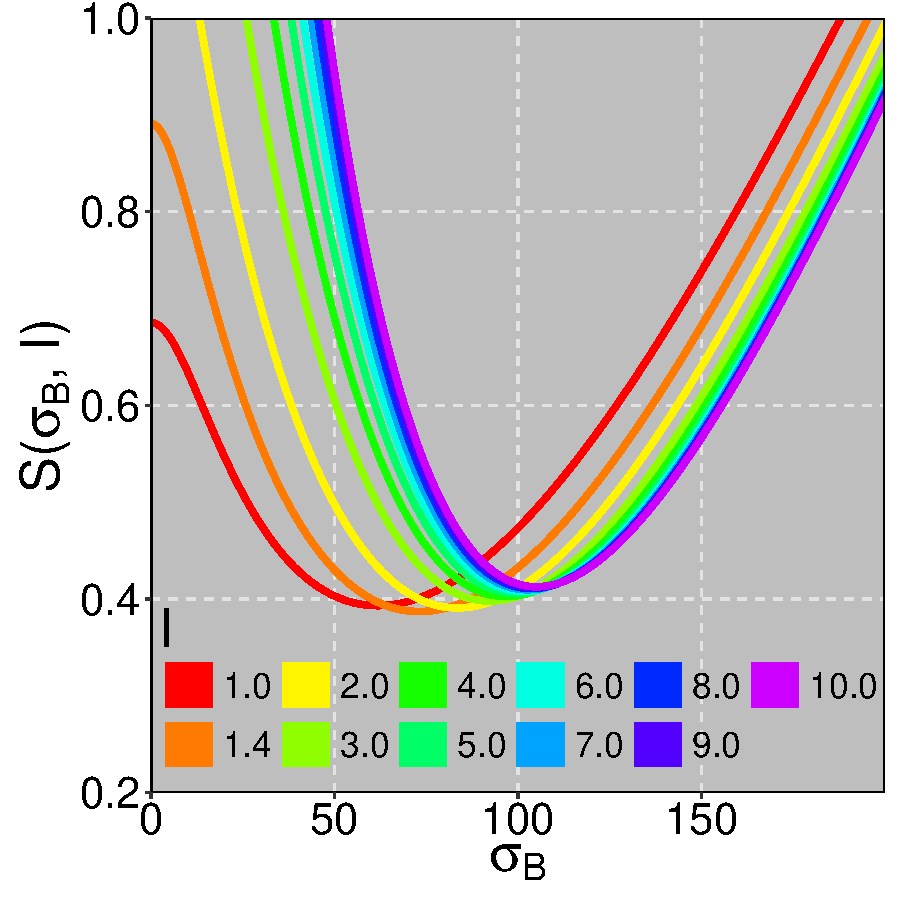
\includegraphics[scale=0.3]{../figures/si_ci_snr_cost_min}
	\caption{Cost function $S(\sigma_B, I)$ from Eq.\ref{eq:cost}.}
	\label{fig:ci_cost}
\end{figure}


\begin{figure}[ht!]
	\centering
	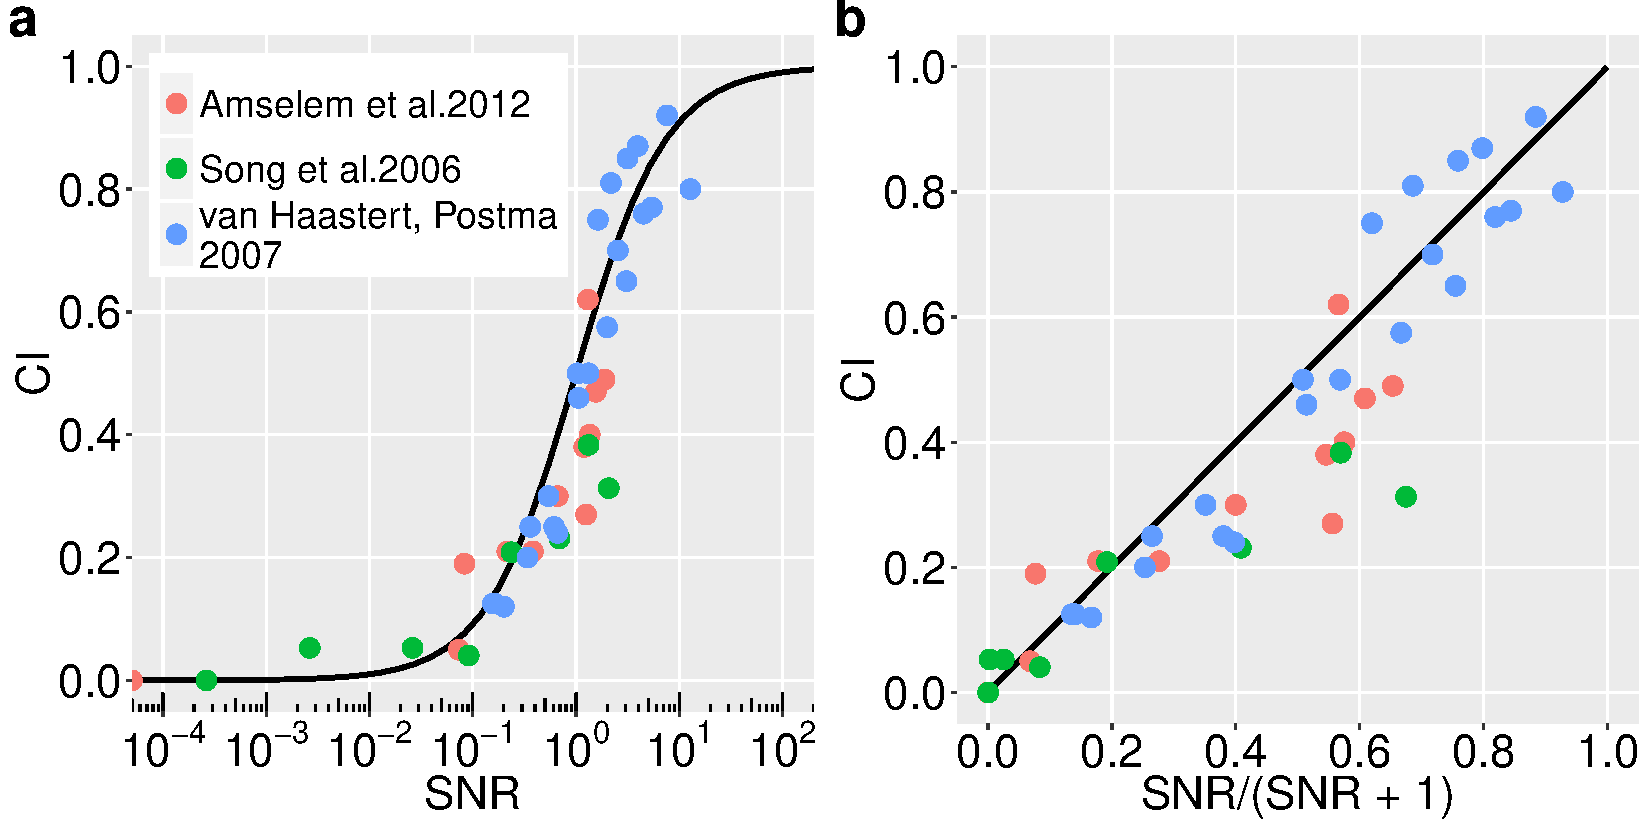
\includegraphics[scale=0.3]{../figures/si_ci_vs_snr_mm_fit}
	\caption{
		Empirical fit to CI, as a function of SNR. SNR was calculated using Eqs.1,2 from the main text and plotted against CI from previous experiments \cite{song, eberhard1, fuller-1} with $\sigma_B = 73$ and $I = 1.4$ fitting parameters.
	}
	\label{fig:ci_vs_snr}
\end{figure}

% Import c0 dcdx CI data from others
\begin{table}[ht]
	\centering
		\begin{tabular}{|c|c|c|c|}
			\hline
			$c_0\,(\mathrm{nM})$ & $|\vec{\nabla}c|\, (\mathrm{nM\,\mu m^{-1}})$ & CI & study \\
			\hline\hline
				 0.0000 & 0.000e+00 & 0.00 & Amselem et al. (2012) \\
				 0.5000 & 3.000e-03 & 0.21 & Amselem et al. (2012) \\
				 5.0000 & 3.000e-02 & 0.38 & Amselem et al. (2012) \\
				15.8000 & 8.000e-02 & 0.47 & Amselem et al. (2012) \\
				25.0000 & 1.000e-01 & 0.62 & Amselem et al. (2012) \\
				50.0000 & 3.000e-01 & 0.49 & Amselem et al. (2012) \\
			 158.0000 & 1.000e+00 & 0.40 & Amselem et al. (2012) \\
			 250.0000 & 1.000e+00 & 0.30 & Amselem et al. (2012) \\
			5000.0000 & 3.000e+01 & 0.19 & Amselem et al. (2012) \\
			 105.0000 & 3.000e-02 & 0.05 & Amselem et al. (2012) \\
				75.0000 & 1.000e-01 & 0.21 & Amselem et al. (2012) \\
				70.0000 & 3.000e-01 & 0.27 & Amselem et al. (2012) \\
				 0.0005 & 3.300e-06 & 0.00 & Song et al. (2006) \\
				 0.0050 & 3.300e-05 & 0.05 & Song et al. (2006) \\
				 0.0500 & 3.300e-04 & 0.05 & Song et al. (2006) \\
				 0.5000 & 3.300e-03 & 0.21 & Song et al. (2006) \\
				 5.0000 & 3.300e-02 & 0.38 & Song et al. (2006) \\
				50.0000 & 3.300e-01 & 0.31 & Song et al. (2006) \\
			 500.0000 & 3.300e+00 & 0.23 & Song et al. (2006) \\
			5000.0000 & 3.300e+01 & 0.04 & Song et al. (2006) \\
				 0.1000 & 2.000e-03 & 0.13 & van Haastert, Postma; pipette (2007) \\
				 0.2000 & 8.000e-03 & 0.25 & van Haastert, Postma; pipette (2007) \\
				 0.4200 & 3.470e-02 & 0.70 & van Haastert, Postma; pipette (2007) \\
				 0.3300 & 2.200e-03 & 0.13 & van Haastert, Postma; pipette (2007) \\
				 0.5000 & 5.000e-03 & 0.25 & van Haastert, Postma; pipette (2007) \\
				 1.0000 & 2.000e-02 & 0.50 & van Haastert, Postma; pipette (2007) \\
				 2.0000 & 8.000e-02 & 0.76 & van Haastert, Postma; pipette (2007) \\
				 2.5000 & 1.250e-02 & 0.24 & van Haastert, Postma; pipette (2007) \\
				 3.3300 & 2.220e-02 & 0.46 & van Haastert, Postma; pipette (2007) \\
				 5.0000 & 5.000e-02 & 0.58 & van Haastert, Postma; pipette (2007) \\
				 6.6700 & 8.890e-02 & 0.65 & van Haastert, Postma; pipette (2007) \\
				10.0000 & 2.000e-01 & 0.77 & van Haastert, Postma; pipette (2007) \\
				20.0000 & 8.000e-01 & 0.80 & van Haastert, Postma; pipette (2007) \\
				 5.0000 & 5.000e-03 & 0.12 & van Haastert, Postma; pipette (2007) \\
				 7.1400 & 1.020e-02 & 0.20 & van Haastert, Postma; pipette (2007) \\
				10.0000 & 2.000e-02 & 0.30 & van Haastert, Postma; pipette (2007) \\
				16.6700 & 5.560e-02 & 0.50 & van Haastert, Postma; pipette (2007) \\
				25.0000 & 1.250e-01 & 0.75 & van Haastert, Postma; pipette (2007) \\
				33.3300 & 2.222e-01 & 0.81 & van Haastert, Postma; pipette (2007) \\
				50.0000 & 5.000e-01 & 0.85 & van Haastert, Postma; pipette (2007) \\
				66.6700 & 8.889e-01 & 0.87 & van Haastert, Postma; pipette (2007) \\
			 200.0000 & 8.000e+00 & 0.92 & van Haastert, Postma; pipette (2007) \\
			\hline
		\end{tabular}
	\caption{Chemotaxis index CI for combinations of mean concentrations and gradients
	used in previous work \cite{song, SNRvh, eberhard1}. For Song et al. \cite{song}
	CI was calculated as the ratio of the velocity in the gradient direction and motility speed $\mathrm{CI} = v_y/v$.
	}
	\label{tab:ci_snr_others}
\end{table}




\section{Reaction-diffusion equations for all models}


Consider a system of two interacting molecules, a small molecule cAMP can be bound by a much larger protein, cAMP phosphodiesterase, which breaks a phosphodiester bond on cAMP and converts it to (5')AMP. This process was shown to be \emph{in-vitro} well described by Michaelis-Menten kinetics \cite{KmcAMPPDEandPDI}:
\begin{equation}
	\mathrm{PDE+cAMP}\overset{k_{1}}{\underset{k_{-1}}{\rightleftharpoons}}C_{cp}\overset{k_{2}}{\rightharpoonup}\mathrm{PDE+5'AMP}
	\label{eq:PDEcAMPint}
\end{equation}
The concentrations of cAMP $c(\vec{r},t)$, PDE $p(\vec{r},t)$, cAMP-PDE complex
$C_{cp}(\vec{r},t)$ and the 5'AMP $c'(\vec{r},t)$ follow the following dynamical equations:
\begin{eqnarray}
	\frac{\partial c}{\partial t} & = & D_c \nabla^2 c - k_1 cp + k_{-1} C_{cp} \label{eq:pdes_full_c}\\
	\frac{\partial p}{\partial t} & = & D_p \nabla^2 p - k_1 cp + (k_{-1} + k_2) C_{cp} \label{eq:pdes_full_p}\\
	\frac{\partial C_{cp}}{\partial t} & = & D_{C_{cp}} \nabla^2 C_{cp} + k_1cp - (k_{-1} + k_2)C_{cp} \label{eq:pdes_full_Ccp}\\
	\frac{\partial c'}{\partial t} & = & D_{c'} \nabla^2 c' + k_2 C_{cp} \label{eq:pdes_full_A}
\end{eqnarray}
We employ a standard quasi-steady-state approximation \cite{QSSA} which sets a concentration scale commonly called a Michaelis-Menten constant $K_M \equiv (k_{-1} + k_2)/k_1$:
\begin{equation}
	k_1 cp = (k_{-1} + k_2)C_{cp},\quad C_{cp} = \frac{cp}{K_M}
\end{equation}
which assumes that the intermediate cAMP-PDE complex does not change on the time scale of product (5'AMP) formation. With this, Eqs.\ref{eq:pdes_full_c}-\ref{eq:pdes_full_A} become:
\begin{eqnarray}
	\frac{\partial c}{\partial t} & = & D_c \nabla^2 c - k_2 C_{cp} = D_c \nabla^2 c - \frac{k_2}{K_M} cp \label{eq:pdes_qssa_c}\\
	\frac{\partial p}{\partial t} & = & D_p \nabla^2 p \label{eq:pdes_qssa_p}\\
	\frac{\partial C_{cp}}{\partial t} & = & D_{C_{cp}} \nabla^2 C_{cp} \label{eq:pdes_qssa_Ccp}\\
	\frac{\partial c'}{\partial t} & = & D_{c'} \nabla^2 c' + \frac{k_2}{K_M} cp \label{eq:pdes_qssa_c'}
		\label{eq:pde_qssa}
\end{eqnarray}
The two relevant equations for cAMP $c(\vec{r},t)$ and PDE $p(\vec{r},t)$ further simplify in steady state:
\begin{eqnarray}
	D_c \nabla^2 c - \frac{k_2}{K_M} cp & = & 0 \\
	D_p \nabla^2 p & = & 0
\end{eqnarray}


\section{Simulation geometry and boundary conditions}


Here we describe the geometry used for both Fixed PDE secretion flux and Fixed PDE concentration models (Fig.\ref{fig:domain}). For both models the outer domain boundaries are set at fixed concentrations (zero for PDE and constant values for cAMP). This reflects recent quantitative efforts to measure cell chemotaxis in microfluidic devices \cite{song, eberhard1, fuller-1}

The cell is modeled as a hemispherical cap placed at the bottom boundary in the $z$ direction. In the first fixed PDE secretion flux model, we set the constant normal PDE flux from the hemispherical surface and zero normal cAMP flux (due to the equilibrium between cAMP binding and unbinding processes, as discussed in the main text). The Fixed PDE concentration model in the main text was solved analytically and these results were verified numerically by having the same boundary conditions as the Fixed PDE secretion flux model except for the zero normal PDE flux on the hemispherical cap. 

\begin{figure}[ht!]
	\centering
	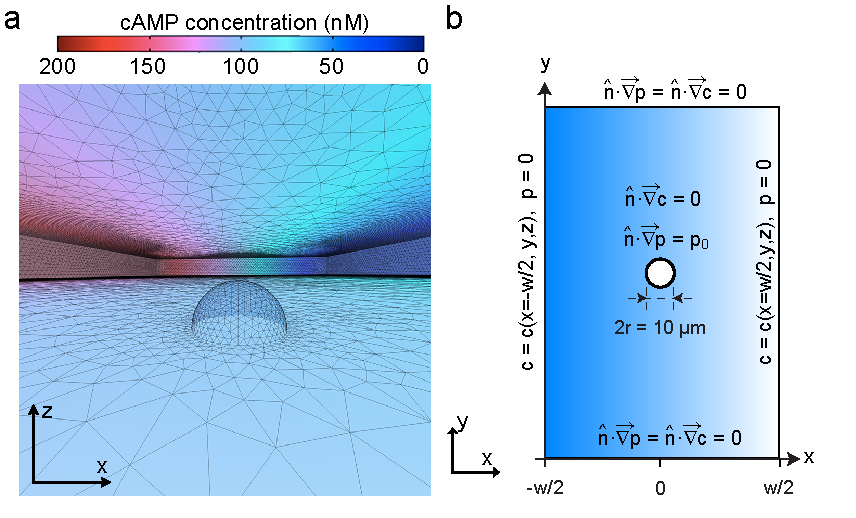
\includegraphics[scale=0.67]{../figures/si_comsol_geometry}
	\caption{
	Simulation geometry. 
	\textbf{a.} Rectangular domain representing microfluidic
	device ($1\mathrm{mm}\times2\mathrm{mm}\times0.1\mathrm{mm}$) and
	a cell modeled as a hemispherical cap (radius $5\,\mu\mathrm{m}$).
	cAMP concentration is color-coded, black lines show the intersections
	of volumetric mesh elements (for the finite element method) with boundaries.
	\textbf{b.} Boundary conditions are fixed concentrations at the sides
	of the device and zero normal flux (reflective) boundaries at the
	top and the bottom. The boundary conditions on the hemispherical cap
	are zero normal flux for cAMP and a constant normal outward flux for
	PDE. Not shown to scale.}
	\label{fig:domain}
\end{figure}


\section{Estimates of model parameters}


\subsection{PDE diffusion coefficient $D_p$}

Diffusion coefficient for PDE was estimated using the Stokes-Einstein
equation for spherical particles \cite{diffusion} following the approach by Tyn and
Gusek \cite{diffusion2}, who provided the following equation
for globular proteins: 
\begin{equation}
	D[\mathrm{cm^2/s}] = \frac{9.2\cdot10^{-8}T[\mathrm{K}]}{\eta[\mathrm{mPas}]\cdot\left(M_r[\mathrm{Da}]\right)^{1/3}}
\end{equation}
where $T[\mathrm{K}]$ is the absolute temperature in Kelvins, $\eta_{\mathrm{water}}^{T=293.15K}=1\,\mathrm{mPas}$ is the dynamic viscosity of water at $20^{\circ}\mathrm{C}$ and $M_{r}[\mathrm{Da}]$ molecular mass. The PDE which has a molecular mass $M_r = 57,500$ Da, then has an estimated diffusion coefficient of $D_p = 70\,\mathrm{\mu m^{2}s^{-1}}$.

\subsection{cAMP-PDE turnover number $k_2$}

We estimated the turnover number $k_{2}$, from \cite{k2paper,pde-purification}
using $k_{2}=V_{max}/p_{0}$, where $V_{max}$ is the maximum rate
of 5'AMP production and $p_0$ is the PDE concentration present. The
PDE concentration present in \cite{pde-purification} was approximately:
\[
p_{0}=\frac{n}{V}=\frac{m/M_{r}}{V}=\frac{6\cdot10^{-4}g}{2\, l\cdot57,500\, g/\mathrm{mol}}\approx\frac{1\cdot10^{-8}\,\mathrm{mol}}{2\, l}=5\,\mathrm{nM}
\]
from $8\cdot10^{10}$ cells. Therefore, since in \cite{k2paper} authors
estimated $V_{max}=10^{-4}\,\mathrm{M/min}$ from $2\cdot10^{9}$
cells, we estimated that the PDE concentration was proportionally
lower: $p_{0}=(2\cdot10^{9}\,\mathrm{cells}\cdot5\,\mathrm{nM})/(8\cdot10^{10}\,\mathrm{cells})$
which gives us $p_{0}=0.125\,\mathrm{nM}.$ We then used this PDE
concentration and $V_{max}$ to estimate the turnover number: 
\begin{equation}
	k_2 = \frac{V_{max}}{p_0} = 13,300\,\mathrm{s^{-1}}
\end{equation}

\subsection{PDE secretion flux $P_0$}

In Fig.1 of \cite{PdePdiKd}, the slope for the PDE activity gives
100 units/ml, and the text gives 2150 units = 0.31 nmol of PDE, so
1 unit of activity corresponds to $1.44\cdot10^{-2}$ nmol of PDE.
Therefore the secretion rate for the entire sample was: 
\begin{eqnarray*}
	\frac{dp_0}{dt} & = & \frac{1.44\cdot10^{1-9}\,\mathrm{mol}/l}{50\,\mathrm{hr}}\cdot0.7\, l \\
			 & = & 5.6\cdot10^{-14}\mathrm{mol\, s^{-1}}
\end{eqnarray*}
Now we assume the PDE flux is uniform through the entire hemispherical
surface of the cell with the radius $5\,\mathrm{\mu m}$, and given
the total of $N_{C}=2.6\cdot10^{7}$ cells, the PDE secretion flux
per cell (secretion rate per cell area) is: 
\begin{eqnarray*}
	P_0 & = & \frac{dp_0/dt}{2\pi r^{2}\cdot N_C} \\
      & = & \frac{5.6\cdot10^{-14}\mathrm{mol\, s^{-1}}}{2\pi(5\mathrm{\mu m})^{2}\cdot2.6\cdot10^{7}} \\
	    & = & 1.4\cdot10^{-11}\mathrm{mol\, m^{-2}s^{-1}}
\end{eqnarray*}


\newpage


\section{Fixed PDE secretion flux model: additional results}


In addition to the applied relative gradient where $c(w/2)=0$ and $c(-w/2)$ was varied, we also performed simulations with either constant applied absolute gradient $|\vec{\nabla}c|_{\mathrm{app}}$ or the midpoint concentration $c_{0, \mathrm{app}}$. The constant $|\vec{\nabla}c|_{\mathrm{app}}$ was simulated by simultaneously changing $c(-w/2)$ and $c(w/2)$ such that $|\vec{\nabla}c|_{\mathrm{app}} = [c(-w/2) - c(w/2)]/w = \mathrm{const}$. The constant $c_{0, \mathrm{app}}$ was simulated similarly but with the constraint $c_{0, \mathrm{app}} = [c(-w/2) + c(w/2)]/2 = \mathrm{const}$. The SNR can again be improved by PDE in both cases.

\subsection{Constant absolute gradient $|\vec{\nabla}c|_{\mathrm{app}}$}

For constant gradient, there is a lower limit on the midpoint concentration $c_0$ due to the finite width of the simulation domain and the fact that $c(w/2) = c_{0, \mathrm{app}} - |\vec{\nabla}c|_{\mathrm{app}}w/2 \geq 0$, so $c_{0, \mathrm{app}} \geq w|\vec{\nabla} c|_{\mathrm{app}}/2$. The results are shown in Fig.\ref{sifig:fixed_dcdx}.

\begin{figure}[!ht]
	\centering
	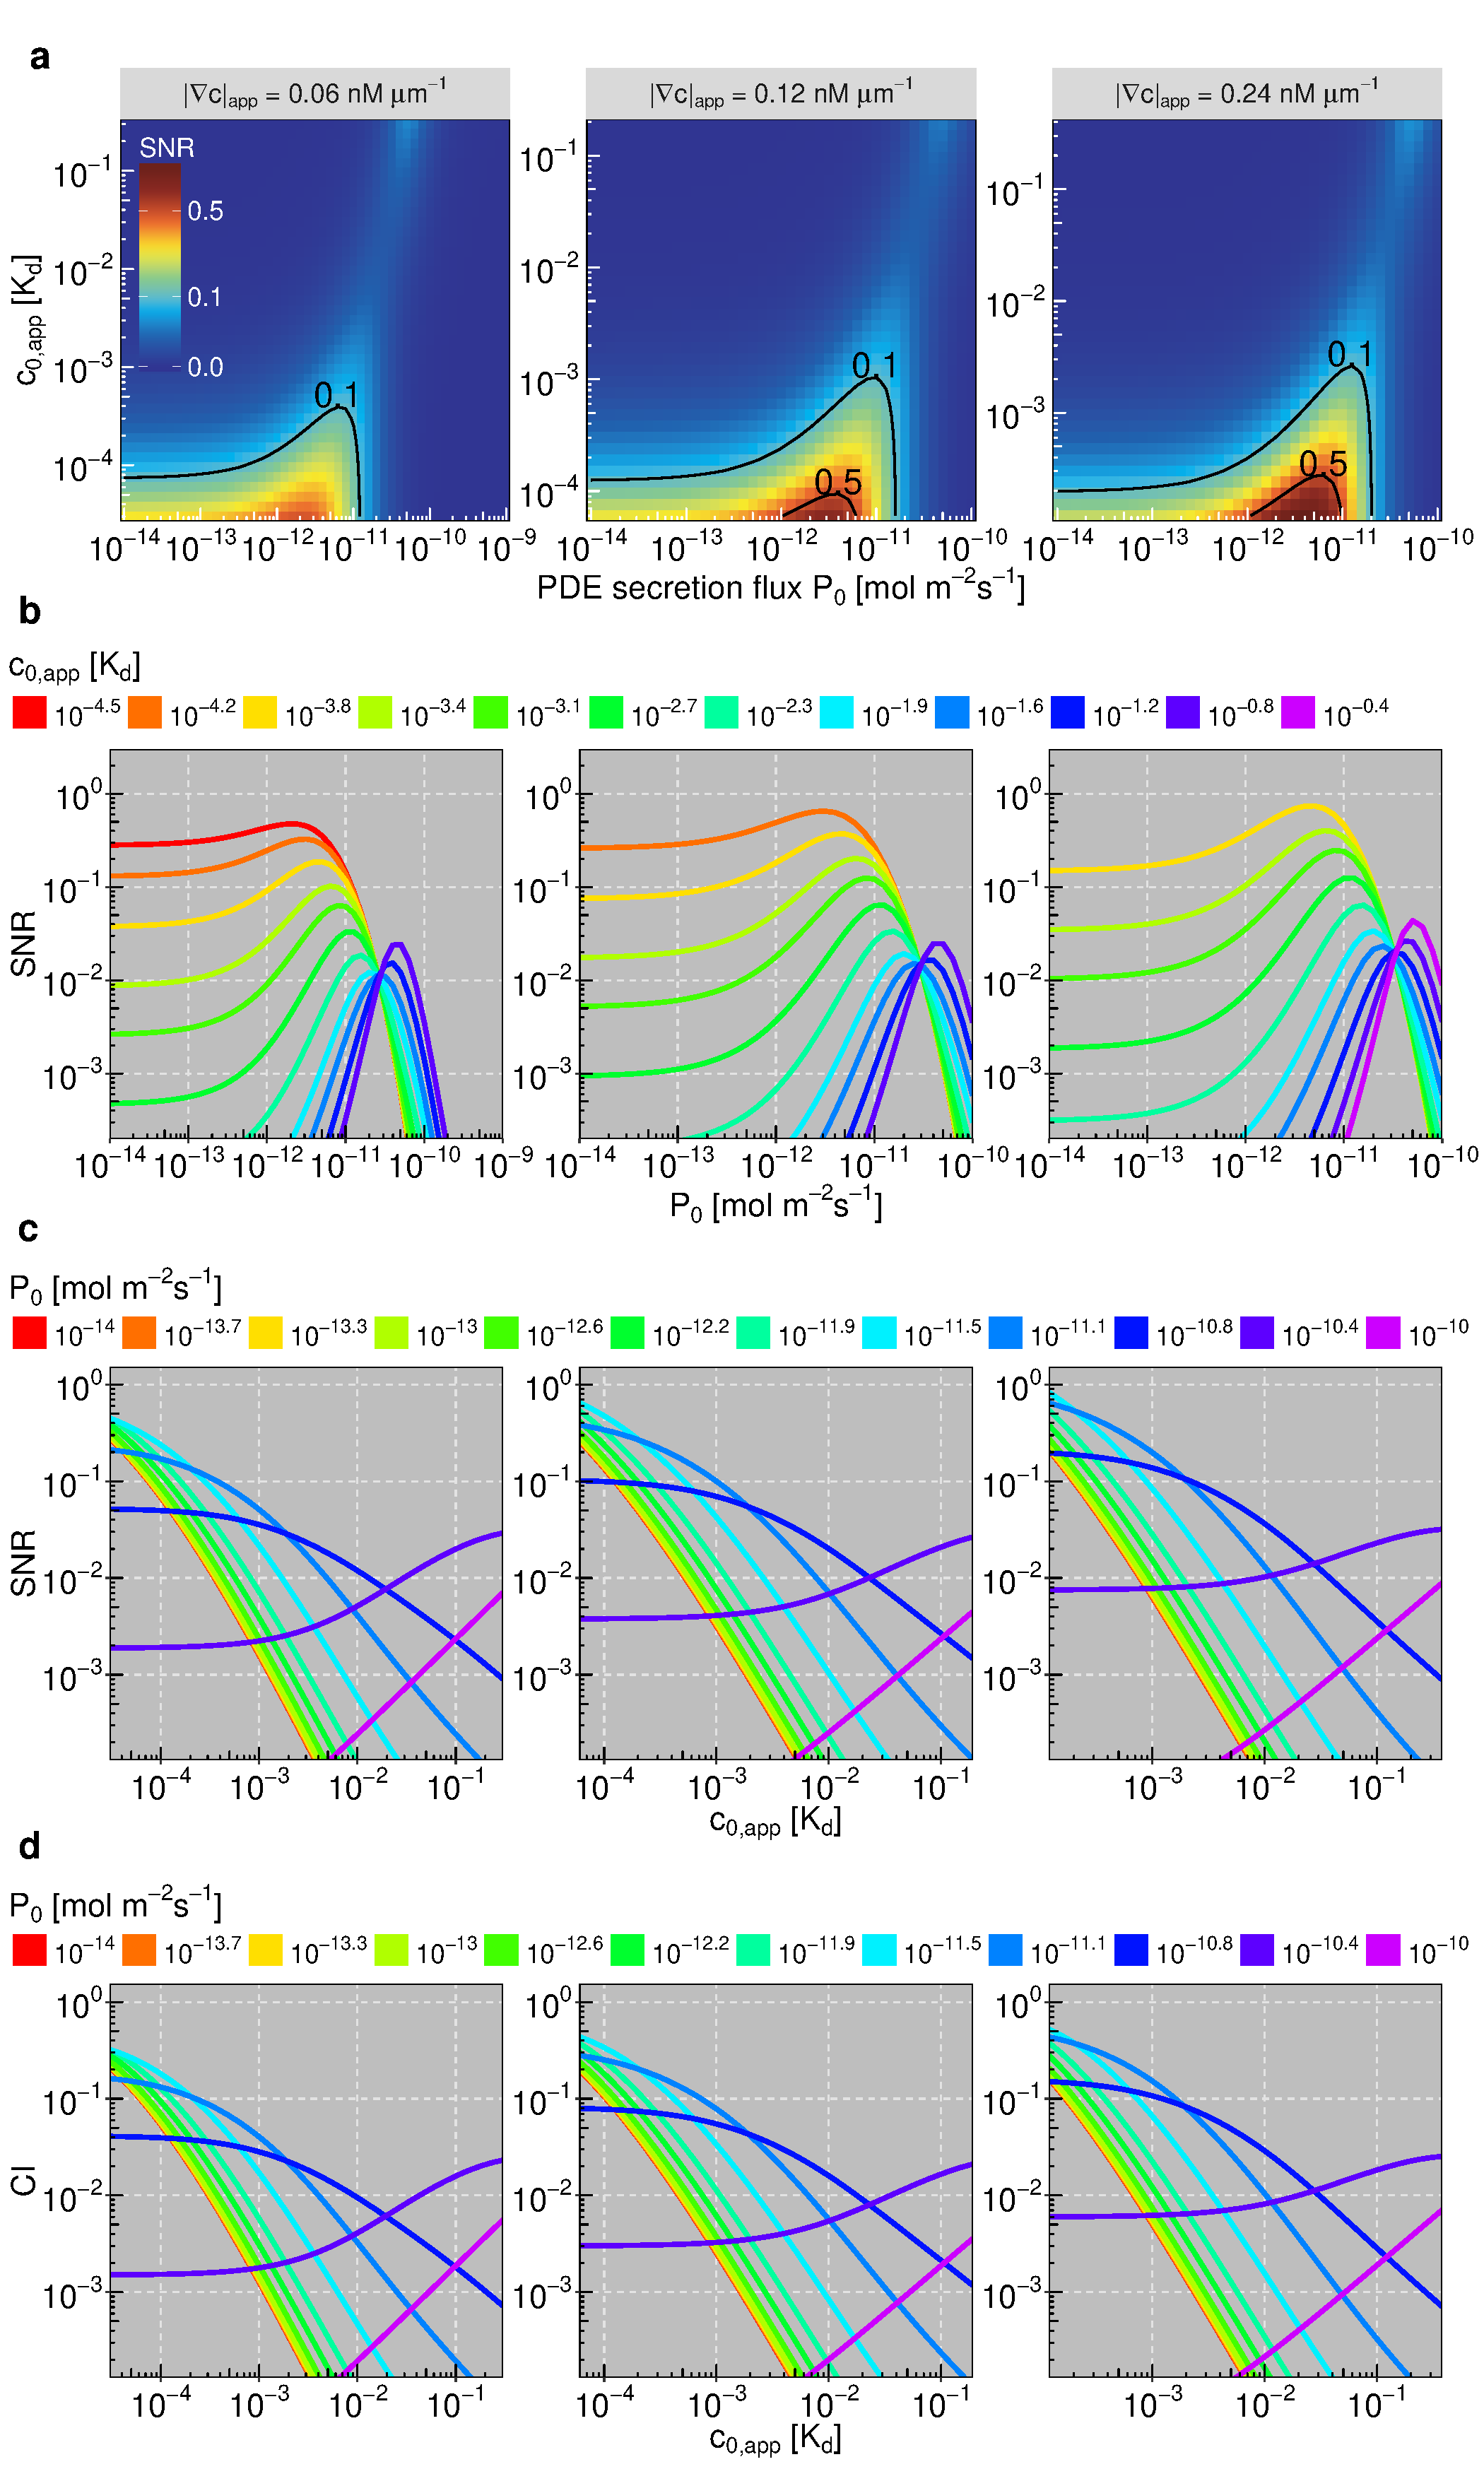
\includegraphics[scale=0.25]{../figures/si_pde_flux_fixed_dcdx_snr_plots}
	\caption{
	Fixed PDE secretion flux model with fixed absolute gradient $|\vec{\nabla}c|_{\mathrm{app}} = 0.06,\,0.12\:\mathrm{or}\:0.24\:\mathrm{nM}\,\mu m^{-1}$. 
	\textbf{a}. SNR as a function of the midpoint concentration $c_0$ and PDE secretion flux $P_0$.
	\textbf{b}. Horizontal slices from a.
	\textbf{c}. Vertical slices from a.
	\textbf{d}. CI as a function of $c_{0,\mathrm{app}}$. The straight lines for low $P_0$ show $\mathrm{CI} \sim c_{0,\mathrm{app}}^{-2}$ scaling.
	}
	\label{sifig:fixed_dcdx}
\end{figure}

\subsection{Constant midpoint concentration $c_{0, \mathrm{app}}$}

Due to the reasons mentioned above, for fixed $c_{0, \mathrm{app}}$, the possible gradients can also be obtained from $c(w/2) = c_{0,\mathrm{app}} - |\vec{\nabla}c|_{\mathrm{app}}w/2 \geq 0$ which gives the condition $|\vec{\nabla}c|_{\mathrm{app}} \leq 2c_{0,\mathrm{app}}/w$. These results are shown in Fig.\ref{sifig:fixed_c0}.

\begin{figure}[!ht]
	\centering
	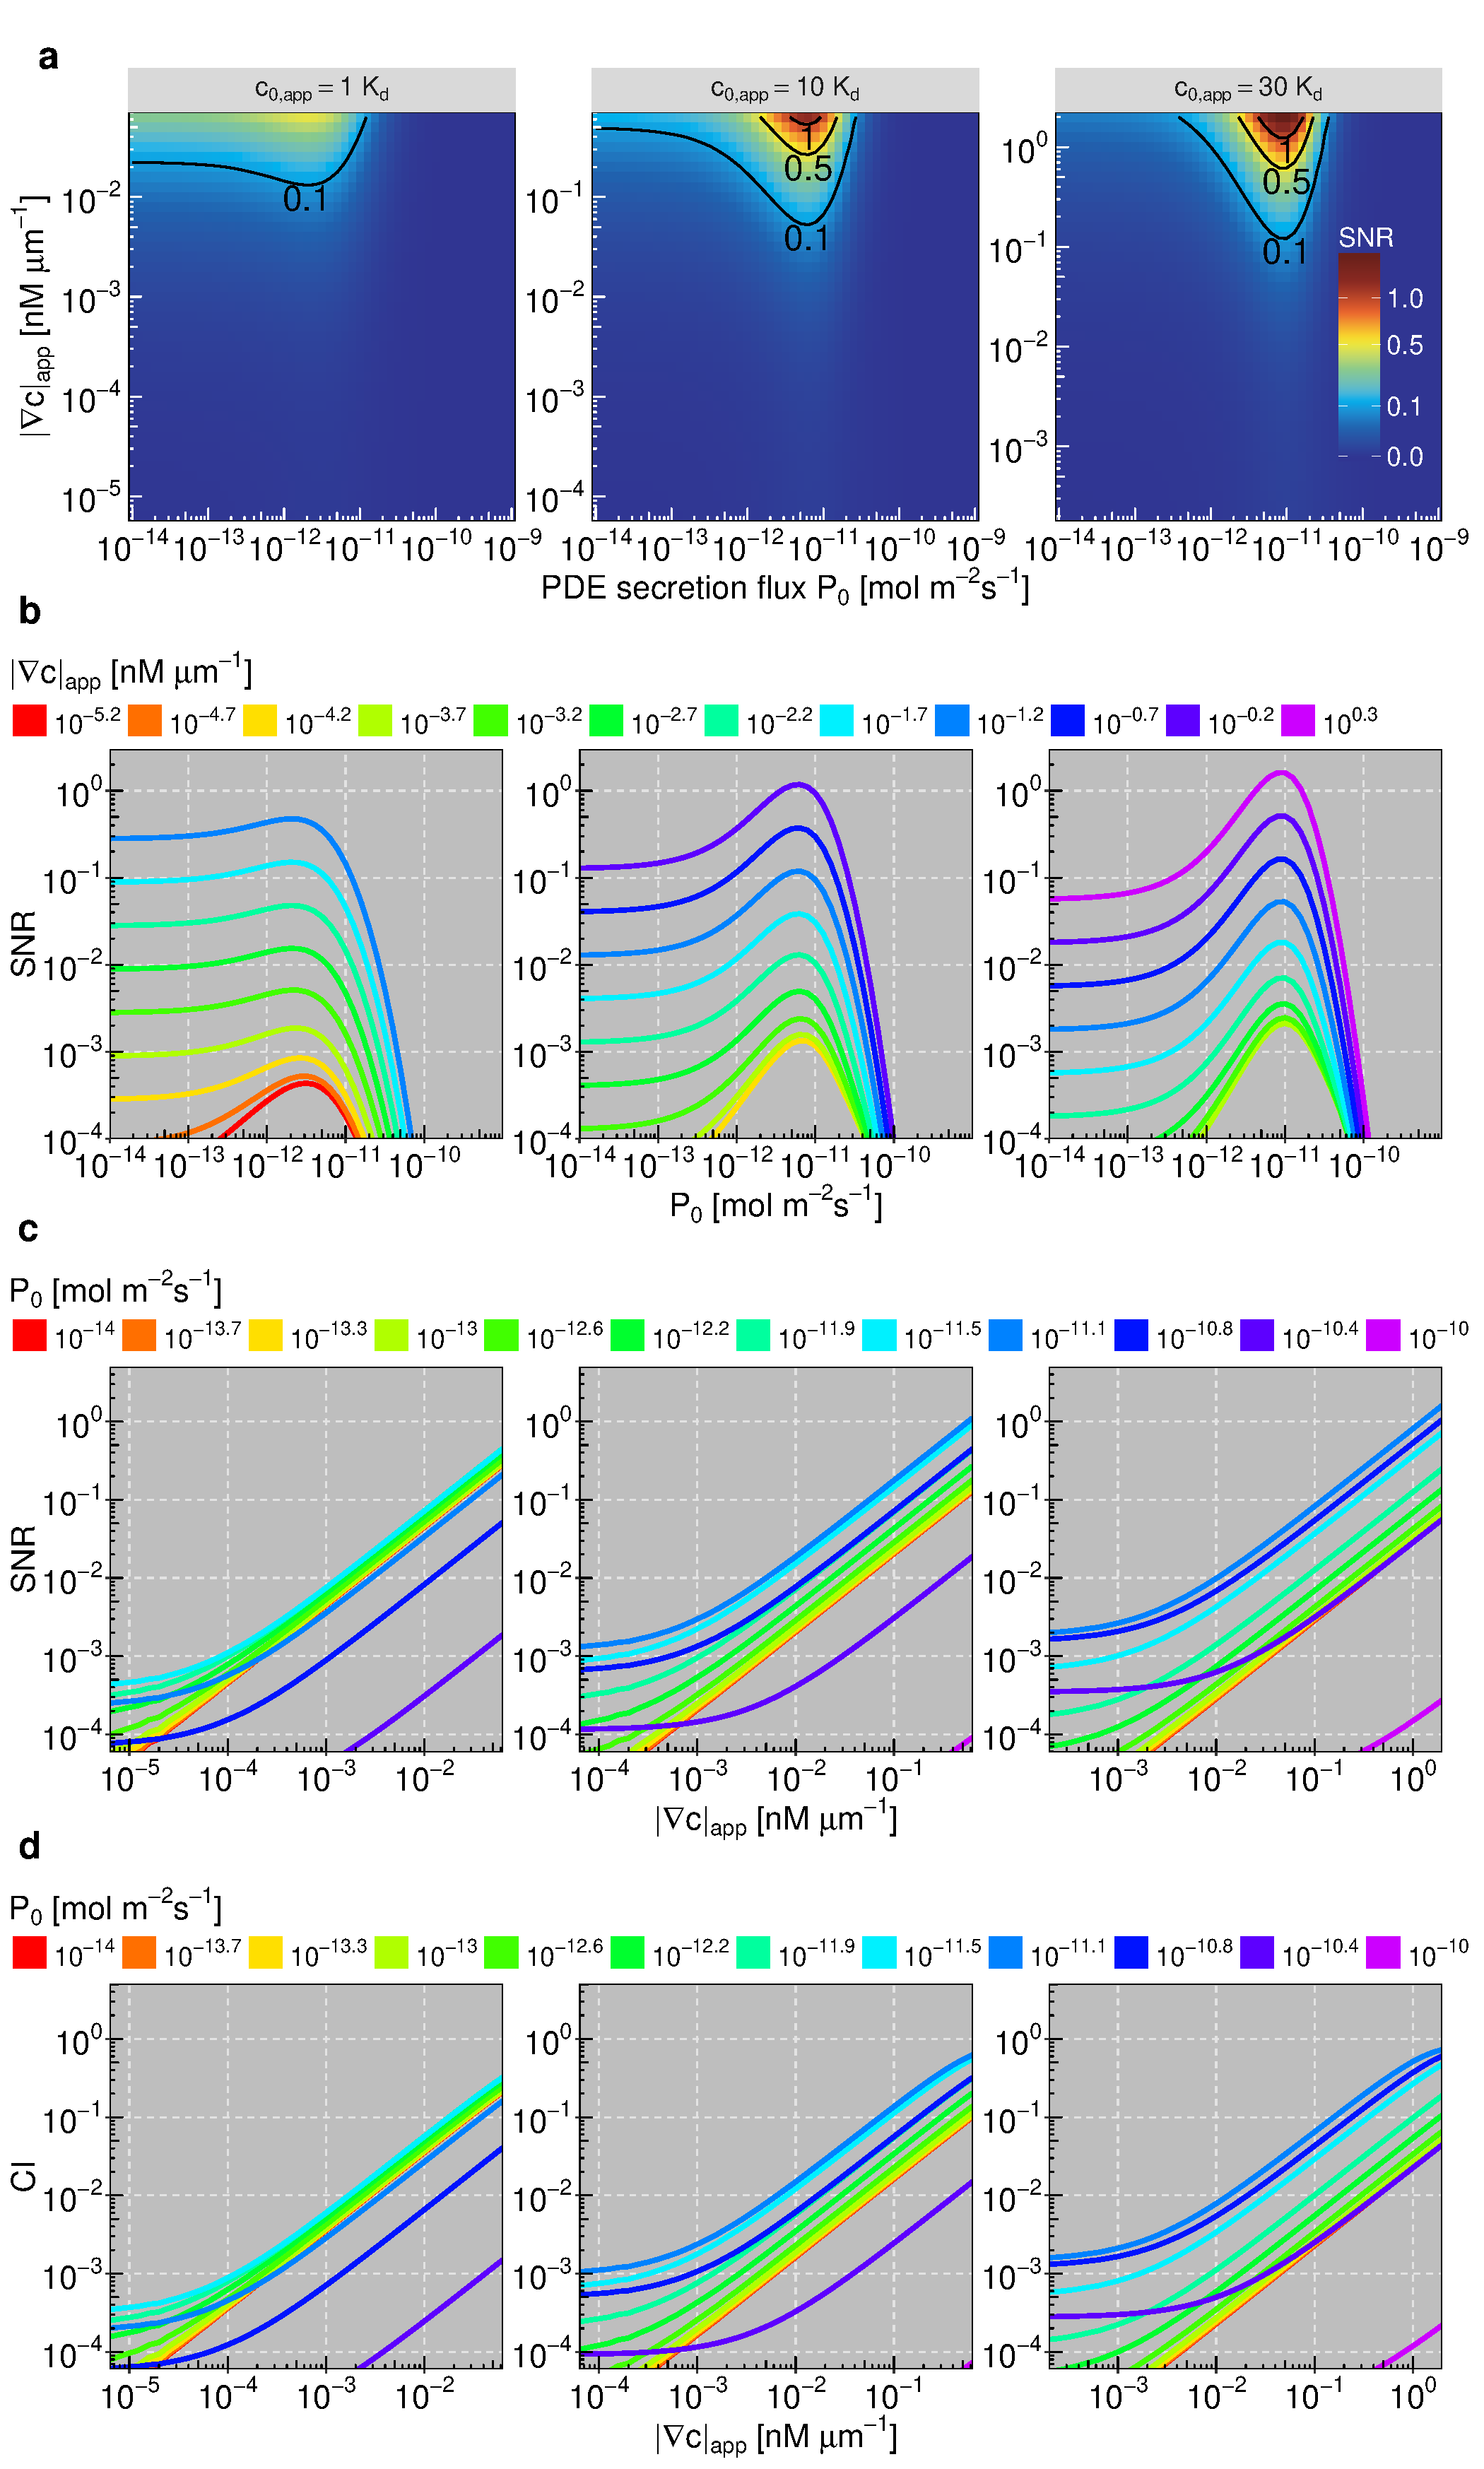
\includegraphics[scale=0.25]{../figures/si_pde_flux_fixed_c0_snr_plots}
	\caption{
	Fixed PDE secretion flux model with fixed midpoint concentration $c_{0,\mathrm{app}} = 1,\,10\:\mathrm{or}\:30\:K_d$. 		
	\textbf{a}. SNR as a function of the applied gradient $|\vec{\nabla}c|_{\mathrm{app}}$ and PDE secretion flux $P_0$.
	\textbf{b}. Horizontal slices from a.
	\textbf{c}. Vertical slices from a.
	\textbf{d}. CI as a function of $|\vec{\nabla}c|$. The straight lines show $\mathrm{CI} \sim |\vec{\nabla}c|_{\mathrm{app}}$ scaling.
	}
	\label{sifig:fixed_c0}
\end{figure}


\newpage


\section{Fixed PDE concentration model $p(\vec{r},t) = p_0$; uniform PDE}


\subsection{Microfluidic geometry}

The solution for cAMP concentration of Eq.5 from the main text
\begin{equation}
		D_c\nabla^{2}c-\frac{k_2p_0}{K_M}c = 0
  \label{eq:main_sys}
\end{equation}
can be solved exactly in a microfluidic geometry by ignoring the height $z$ and length $y$ coordinates:
\begin{equation}
	\frac{d^2c}{dx^2} - \frac{c}{L^2} = 0, \quad
	L=\sqrt{\frac{K_M D_c}{k_2p_0}}
\end{equation}
which has solutions of the form:
\begin{equation}
	c(x) = Ae^{-x/L} + Be^{x/L}
\end{equation}
and with boundary conditions
\begin{equation}
	c(x=-w/2) = c(-w/2), \quad c(x = w/2) = 0 
\end{equation}
becomes:
\begin{equation}
	c(x) = c(-w/2) \frac{\sinh\left(\frac{w}{2L}-\frac{x}{L}\right)}
		{\sinh\left(\frac{w}{L}\right)}
	\label{eq:uniform_pde_analytic_sol}
\end{equation}
The mean concentration and gradient at $x=0$ (where the cell boundary used to be) are:
\begin{equation}
	c_0 = \frac{c(-w/2)}{2\cosh\left(\frac{w}{2L}\right)},\quad |\vec{\nabla} c| = \frac{c(-w/2)}{2L\sinh\left(\frac{w}{2L}\right)}
		\label{eq:pde_uniform_c0_dcdx}
\end{equation}
The analytical expression for SNR can be simplified under the approximation of shallow gradients $r_c|\vec{\nabla}c| \ll K_d$ which is well satisfied in this work ($\mathrm{max}(r_c|\vec{\nabla}c|/K_d) = 5\cdot10^{-3}$) and is obtained from Eq.\ref{eq:pde_uniform_c0_dcdx}:
\begin{equation}
	\mathrm{SNR} \approx \frac{N K_d r_c |\vec{\nabla}c|}{2(c_0 + K_d)\sqrt{\sigma_B^2(c_0 + K_d)^2 + N c_0 K_d}}
\end{equation}
These results are shown in Fig.\ref{fig:uniform_pde_snr}. For the interesting range $p_0 \gg 10^{-3}\,\mathrm{nM}$, it follows that $w \gg 2L$ so we can simplify the Eq.\ref{eq:pde_uniform_c0_dcdx}:
\begin{equation}
	c_0 \approx c(-w/2)e^{-w/2L},\quad |\vec{\nabla}c| \approx \frac{c(-w/2)}{L} e^{-w/2L}
\end{equation}
This shows that even though the applied relative gradient $r_c|\vec{\nabla}c|_{\mathrm{app}}/c_{0,\mathrm{app}} = 2r_c/w$ is constant, the relative gradient across the cell body is not constant and is PDE dependent:
\begin{equation}
	\frac{r_c|\vec{\nabla}c|}{c_0} = \frac{r_c}{L}
\end{equation} 
Therefore, the PDE introduces a new characteristic length $L$ instead of the original $w$. Fig.\ref{fig:uniform_pde_snr} shows that the conclusions drawn from Fixed PDE secretion flux model (Fig.3 in the main text) are the same here.

\begin{figure}[!ht]
	\centering
	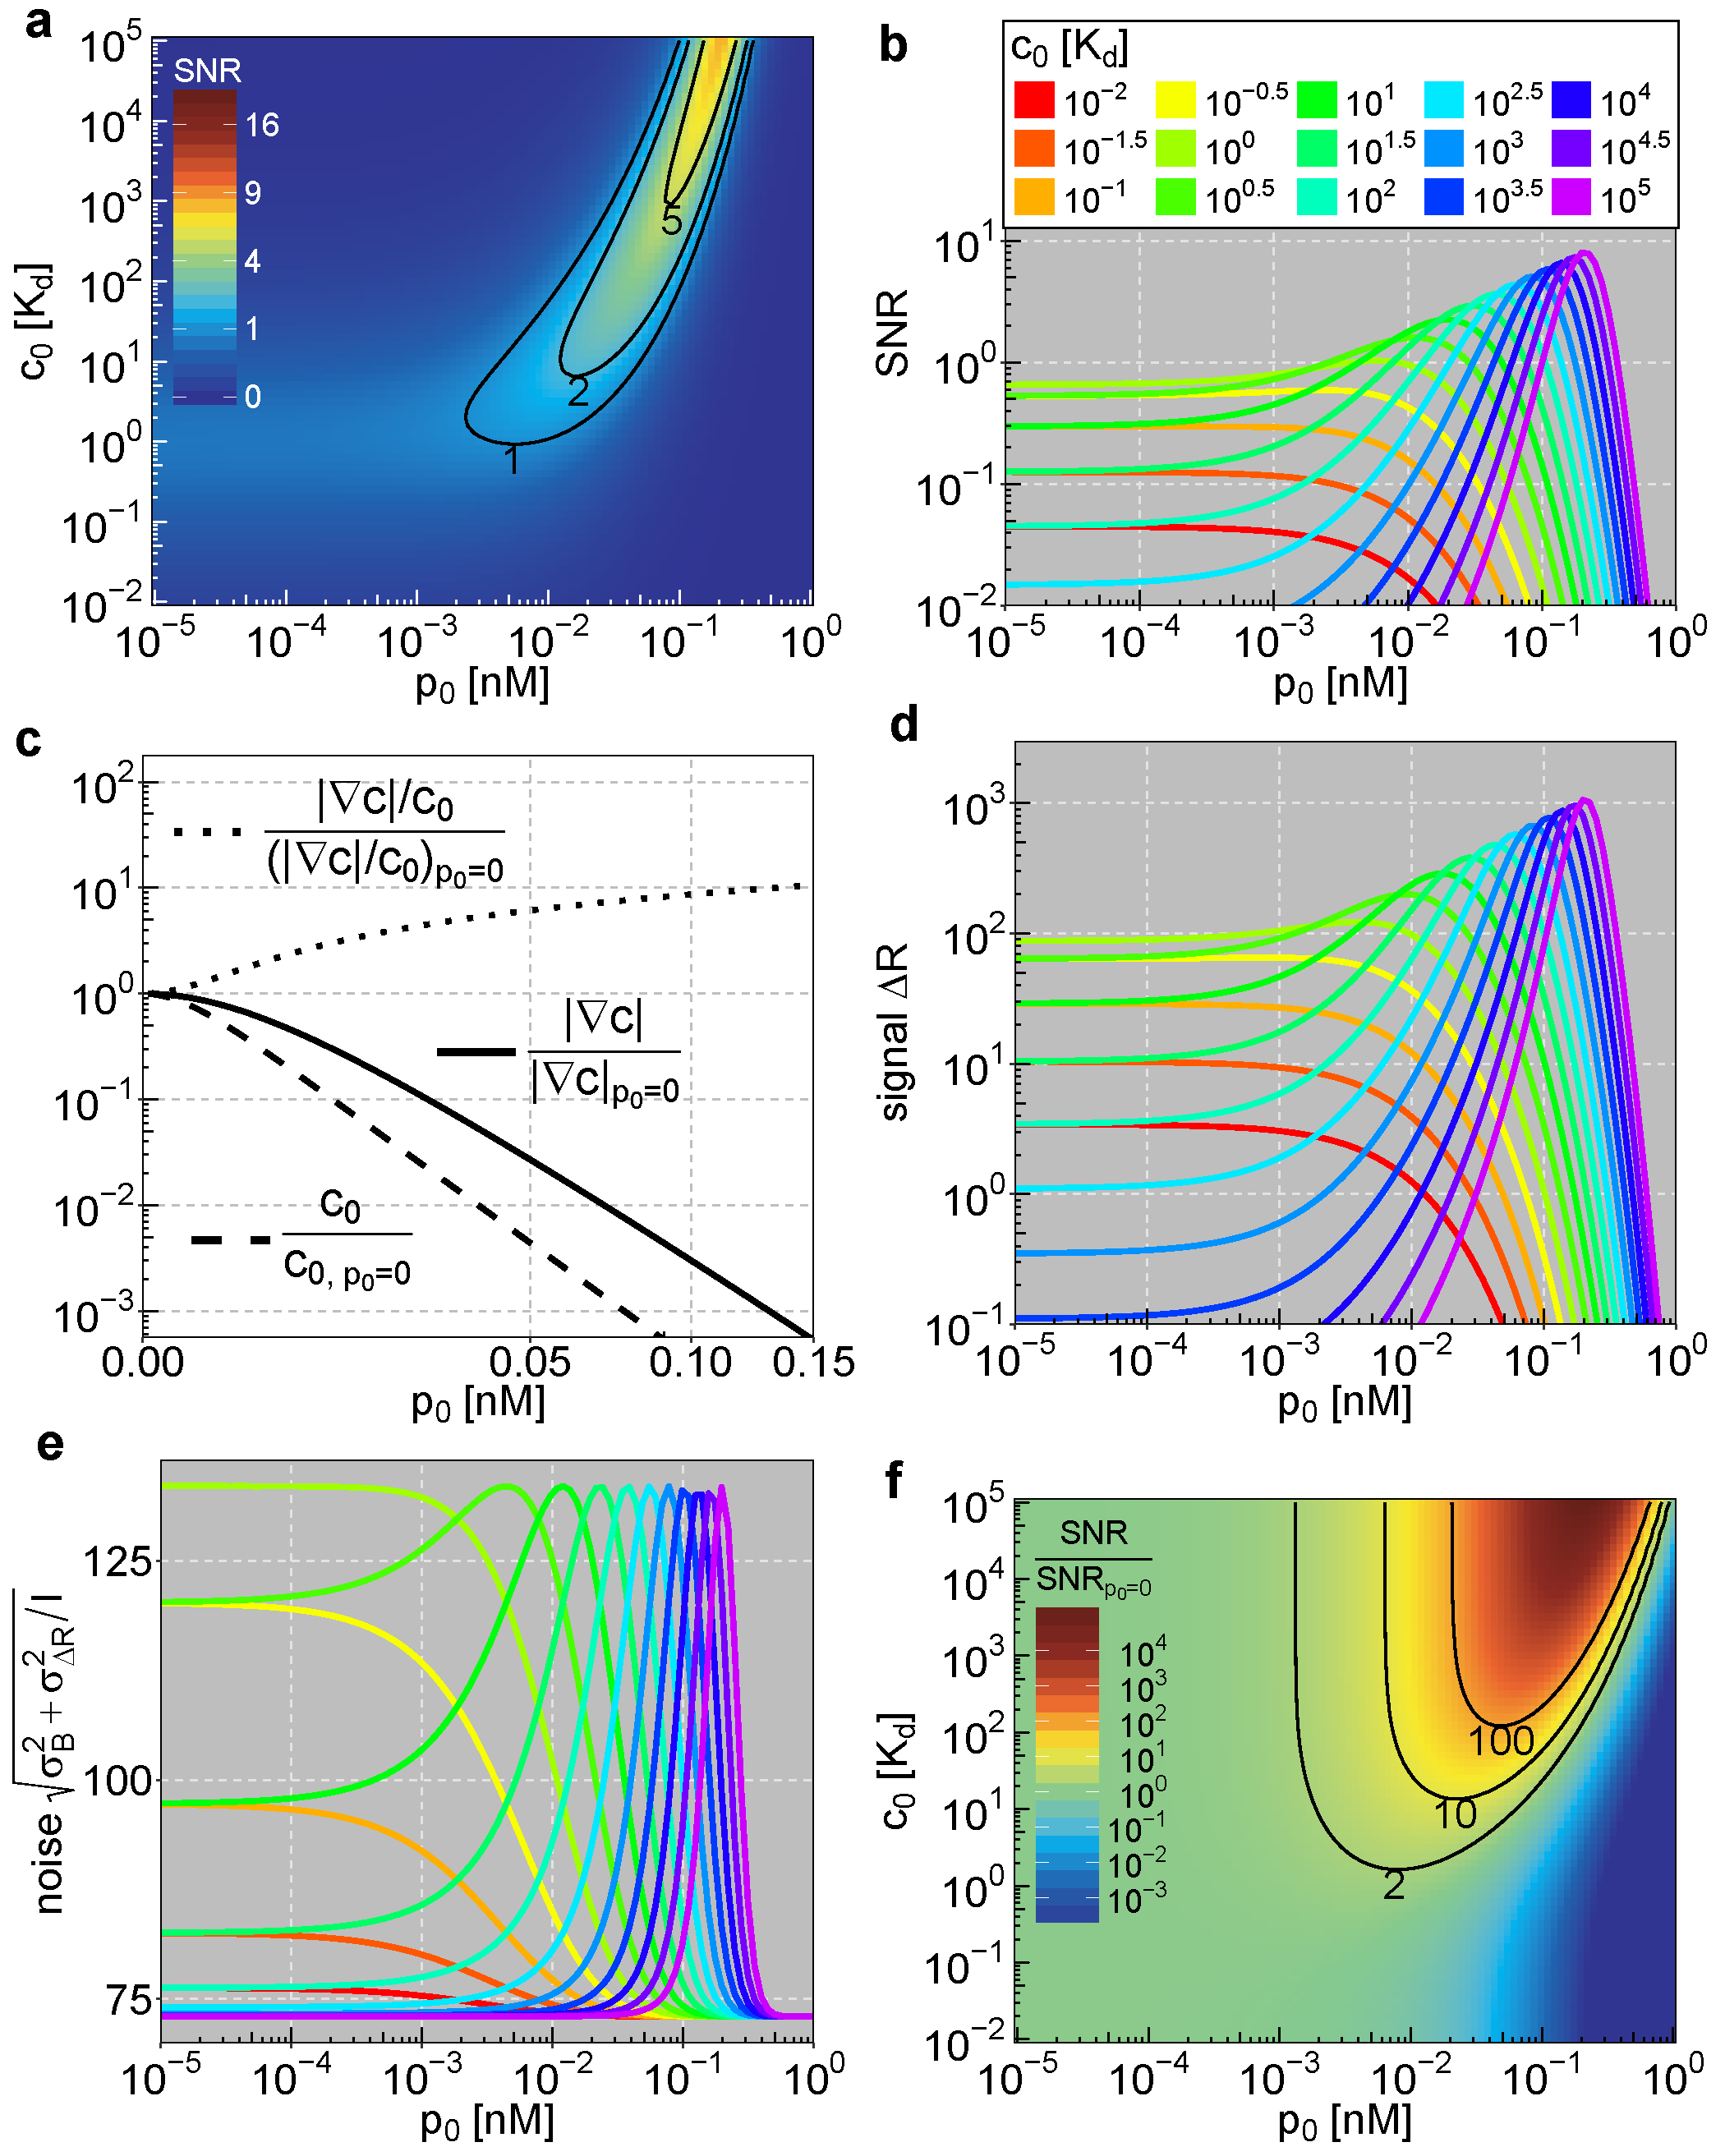
\includegraphics[scale=0.245]{../figures/si_pde_uniform_signal_noise_snr}
	\caption{
		Analytical exact solution for Fixed PDE concentration model, with varying $c(-w/2)$ and $c(w/2)=0$ (as in Figs2,3 in the main text). 
		\textbf{a}. $\mathrm{SNR}(p_0, c(-w/2))$, which shows similar trend to the fixed PDE secretion flux model.
		\textbf{b}. Horizontal slices from a. Same color legend applies also to d and e.
		\textbf{c}. Mean concentration $c_0$, relative gradient $|\vec{\nabla}c|/c_0$ and absolute gradient $|\vec{\nabla}c|$ (relative to their values with $p_0=0$) across the cell body as a function of PDE concentration $p_0$. 
		\textbf{d}. Signal ($\Delta R$) as a function of $p_0$. 
		\textbf{e}. Noise as a function of $p_0$, with lower limit of $\sigma_b = 73$ and upper limit of $\sqrt{\sigma_B^2 + N/(4I)}$.
		\textbf{f}. Ratio of SNR with $p_0 \neq 0$ and SNR with $p_0=0$. 		
	}
	\label{fig:uniform_pde_snr}
\end{figure}



\subsection{Cell boundary effects on SNR}


We analyzed the effect of cell boundary on SNR, by comparing the exact analytical solution of SNR (main text, Fig.3) for the fixed PDE concentration model, to the numerical solution where we have the cell boundary (like in the fixed PDE secretion flux model). The results are shown in Fig.\ref{fig:si3} and show that to a large extent, the only difference is the scaling factor of $\sim 1$.
\begin{figure}[ht!]
	\centering
	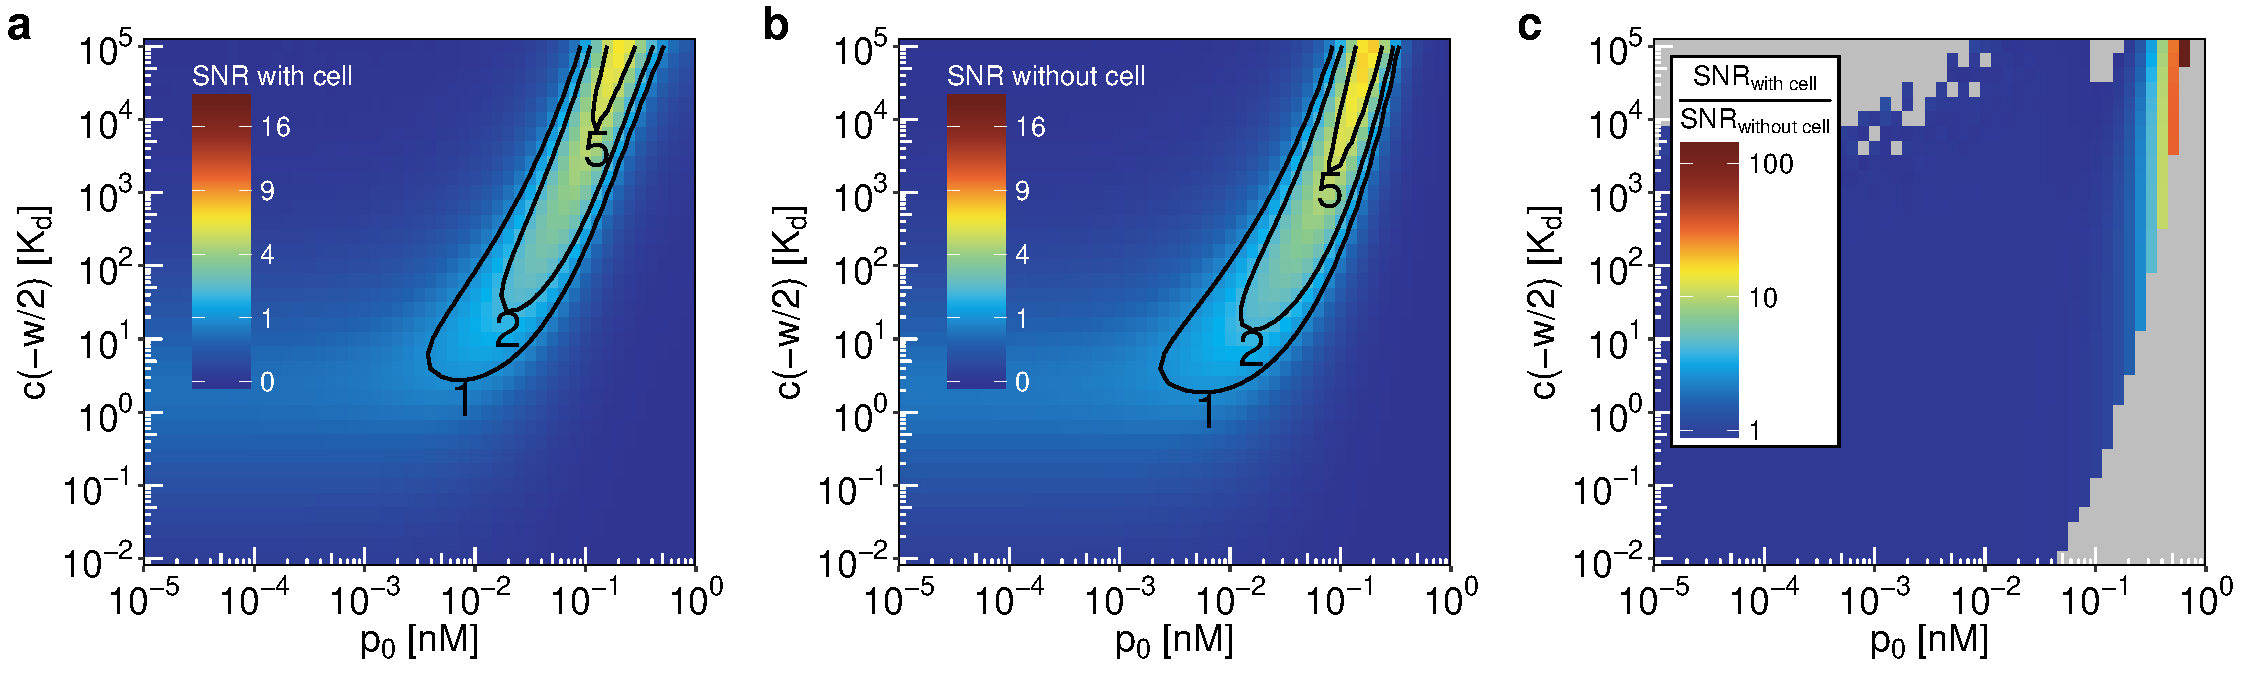
\includegraphics[scale=0.43]{../figures/si_pde_uniform_compare_with_without_cell}
	\caption{
		Effect of cell boundary on the SNR.
		\textbf{a} Exact analytic result for SNR is calculated as in the main text, but only for the combination of $c(-w/2)$ and $p_0$ values from part b.
		\textbf{b} SNR is calculated without the cell boundary in the middle of simulation domain.
		\textbf{c} Ratio of SNR from a to SNR from b. Due to the numerical inaccuracy of the ratio of two small values, only the results for $\mathrm{SNR_{without\ cell}} \geq 10^{-3}$ are shown.
	}
	\label{fig:si3}
\end{figure}


\subsection{cAMP point source, full 3D model}


Here, we analyze the case where the gradient is generated by a point source in 3D (at origin) and the PDE distribution is uniform. In this case the cAMP concentration follows:
\begin{equation}
	\frac{\partial c}{\partial t} = D_c \nabla^2 c - \frac{k_2 p_0}{K_M}c + C_0 \delta(r)
	\label{eq:pdeSpherical}
\end{equation}
where $\delta(r)$ is the delta function and $C_0$ its strength. The steady state equation has the form:
\begin{equation}
	\left(\nabla^2 - \frac{1}{L^2}\right)c(r) = C_0 \delta(r)
\end{equation}
where we again substituted $L = \sqrt{K_M D_c / (k_2 p_0)}$. The solution for cAMP concentration is equivalent to the Green's function for a Screened Poisson equation, which can be obtained by performing a Fourier transform of $c(r)$ and $\delta(r)$:
\begin{equation}
	c(r) = \frac{1}{(2\pi)^3} \int e^{-i\vec{k}\vec{r}} \tilde{c}(\vec{k}) d\vec{k},\quad 
	\delta (r) = \frac{1}{(2\pi)^3} \int e^{-i\vec{k}\vec{r}} d\vec{k}
\end{equation}
\begin{equation}
	\left(-k^2 - \frac{1}{L^2}\right)\tilde{c}(\vec{k}) = C_0
\end{equation}
\begin{equation}
	\tilde{c}(k) = -\frac{C_0}{k^2 + \frac{1}{L^2}}
\end{equation}
where $k = |\vec{k}|$. Now we can reverse Fourier transform to obtain the concentration $c(r)$, so we write $\vec{k}$ in spherical coordinates, choosing the north pole as the direction of $\vec{r}$:
\begin{equation}
	c(r) = - \frac{1}{(2\pi)^3}\int_0^{2\pi} d\phi \int_0^{\pi} d\theta \int_{-\infty}^{\infty} dk C_0 \frac{k^2}{k^2 + \frac{1}{L^2}} e^{ikr\cos\theta} \sin\theta
\end{equation}
Integrating over $\phi$ gives a factor of $2\pi$ and substituting $\cos\theta = \omega$, $d\omega = -\sin\theta d\theta$ we have:
\begin{equation}
	c(r) = \frac{1}{(2\pi)^2} \int_{-\infty}^{\infty} dk \int_1^{-1} d\omega e^{ikr\omega} C_0 \frac{k^2}{k^2 + \frac{1}{L^2}}
\end{equation}
\begin{equation}
	c(r) = \frac{1}{2\pi^2} \int_{-\infty}^{\infty} dk \frac{k^2}{k^2 + \frac{1}{L^2}} \frac{\sin(kr)}{kr}
\end{equation}
now we can integrate over $k$ \cite{wolfram} to get:
\begin{equation}
	c(r) = C_0 \frac{e^{-r/L}}{r}
	\label{eq:spherical_camp}
\end{equation}
where we absorbed $2\pi$ into the constant $C_0$. The Eq.\ref{eq:spherical_camp} is used to calculate the cAMP concentration at a distance $r$ emitted by a point source in 3D at $r = 0$. As before, we plug Eq.\ref{eq:spherical_camp} into equations (1-2) from the main text to calculate SNR. The results are shown in Fig.\ref{fig:snr_spherical_results} and show the same effect of SNR enhancement occurring in this geometry as well.

% Figure SI 5. Spherical model, uniform PDE results.
\begin{figure}
	\centering
	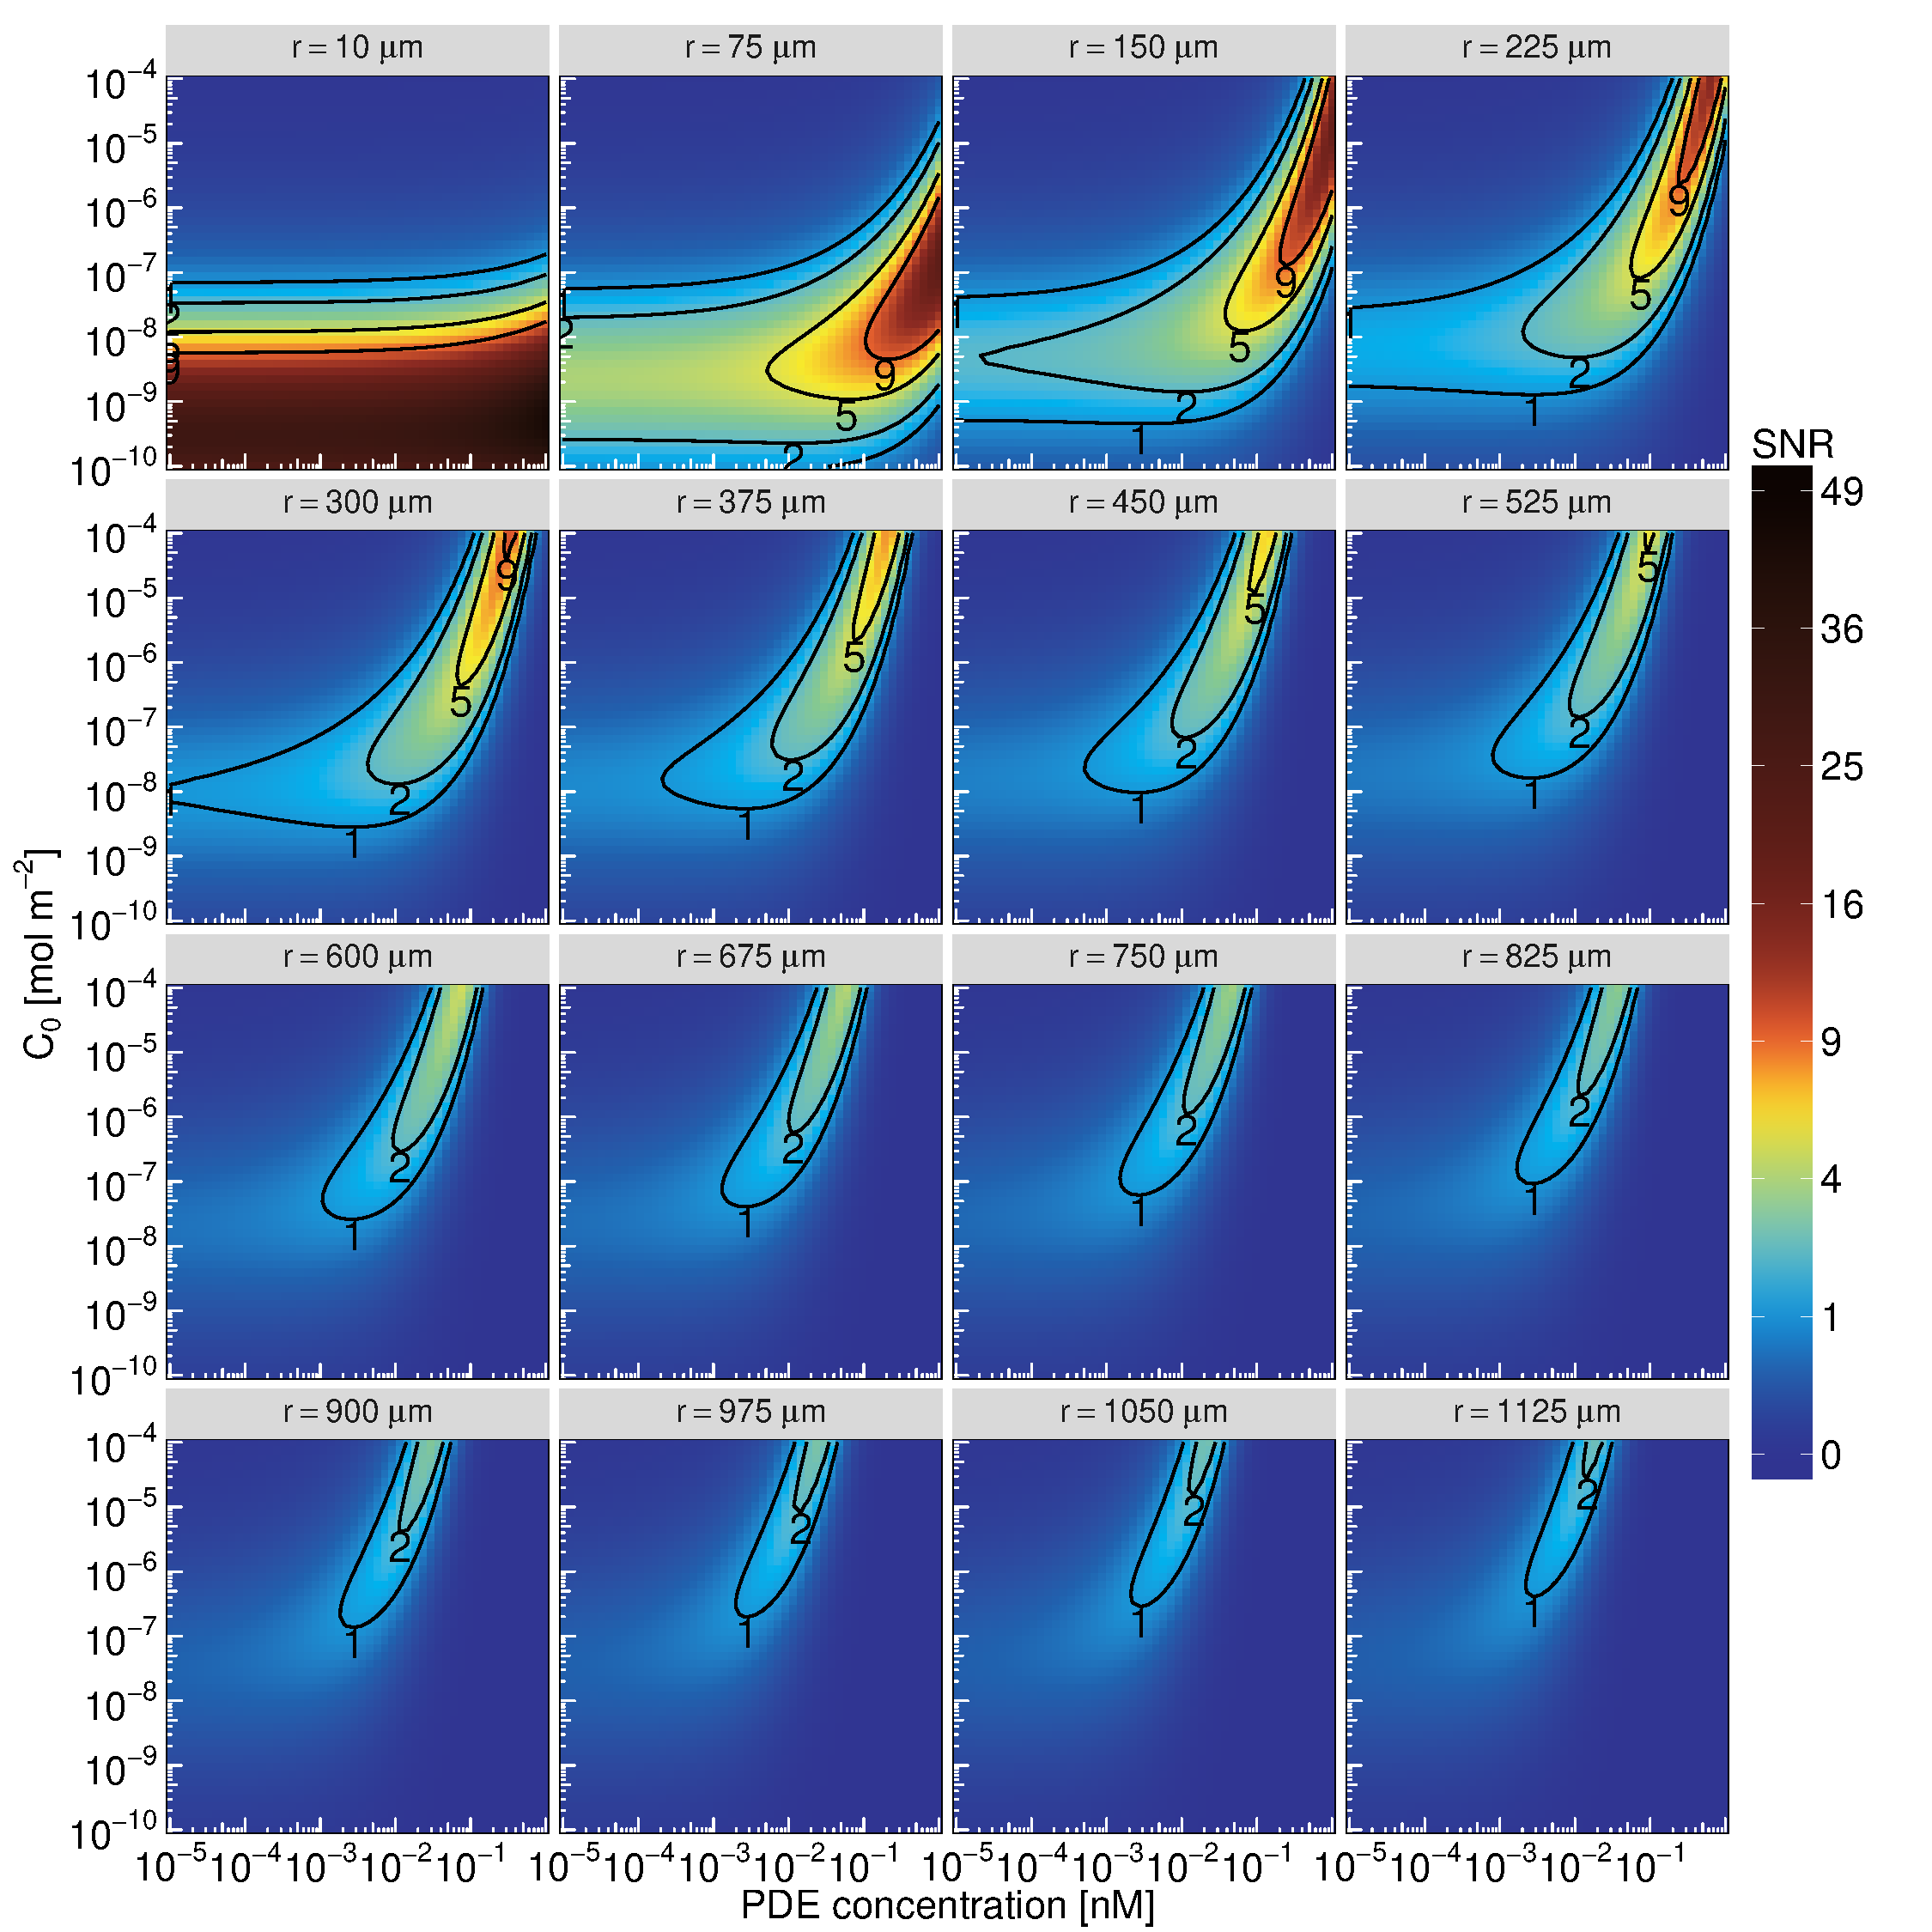
\includegraphics[scale=0.35]{../figures/si_pde_uniform_spherical_model_snr}
	\caption{SNR for a spherical model with the uniform PDE concentration, plotted as a function of PDE concentration $p_0$, the delta function strength $C_0$ (representing the cAMP secretion flux from the point source) and the cell distance from the point source $r$. We observe the same enhancement of SNR as in the models from the main text, up to relatively large distances from the source ($\sim$ 0.5 mm). }
	\label{fig:snr_spherical_results}
\end{figure}


In the case of microfluidic geometry we saw that the net effect of PDE is to convert the original applied relative gradient $\sim r_c/w$ to a new PDE-dependent gradient $\sim r_c/L$ with a shorter characteristic length (and therefore larger relative gradient). Here the absolute gradient is:
\begin{equation}
	|\vec{\nabla}c| = C_0\frac{e^{-r/L}}{r}\left(\frac{1}{r} + \frac{1}{L}\right)
\end{equation}
and the relative gradient across the cell at position $r$ is:
\begin{equation}
	\frac{r_c |\vec{\nabla}c|}{c} = \frac{r_c}{L} + \frac{r_c}{r}
\end{equation}
Here we see the similar effect of PDE. The original relative gradient $r_c/r$ is now increased by an additive term $r_c/L$ proportional to the square root of PDE concentration.

	

%If the cell is located at $r = r_0$ away from the point cAMP source, the concentration and gradient are:
%\begin{equation}
	%\frac{c(r)}{c(r; p_0=0)} = e^{-r/L}
%\end{equation}
%
%\begin{eqnarray}
	%\frac{|\vec{\nabla}c|}{|\vec{\nabla}c|_{p_0 = 0}} & = & \frac{c(r)}{c(r; p_0 = 0)} \frac{\frac{1}{L} + \frac{1}{r}}{\frac{1}{r}} \\
		%& = & e^{-r/L} \frac{\frac{r + L}{rL}}{\frac{1}{r}} \\
		%& = & e^{-r/L} \left(\frac{r}{L} + 1 \right)
%\end{eqnarray}
%
%\begin{eqnarray}
	%|\vec{\nabla}c| & = & C_0 \frac{e^{-r/L}}{r}\left(\frac{1}{L} + \frac{1}{r} \right) \\
		%& = & c(r) \left(\frac{1}{L} + \frac{1}{r} \right)
%\end{eqnarray}




\section{Peclet number analysis of  flow-gradient experiments}


In experiments where cAMP gradients are set up by flow \cite{song, eberhard1, fuller-1}, the average flow speed was $\left\langle v\right\rangle = 650\,\mu\mathrm{m\,s^{-1}}$. Due to the small height of the the microfluidic channel of $h = 50\,\mu\mathrm{m}$ (compared to the length of 5 mm and width of 0.5 mm), the flow can be well described as an incompressible, laminar flow between two infinite fixed parallel horizontal plates where $v(z=0) = v(z=h) = 0$, which has the solution of the form:
\begin{equation}
	v(z) = \alpha z(h - z)
\end{equation}
The proportionality constant $\alpha$ can be calculated from the average speed:
\begin{equation}
	\left\langle v\right\rangle = \frac{1}{h}\int_0^h v(z) dz = \frac{\alpha h^2}{6}
\end{equation}
\begin{equation}
	\alpha = \frac{6 \left\langle v\right\rangle}{h^2} = \frac{1.56}{\mu\mathrm{m\cdot s}}
\end{equation}
Since the cells are attached to the glass bottom of the microfluidic device we can calculate the average flow speed around cell whose height is equal to its hemispherical radius $r_c = 5\,\mu\mathrm{m}$:
\begin{equation}
	v_{\mathrm{cell}} = \left\langle v\right\rangle_{0\leq z \leq r_c} = \frac{1}{r_c} \int_0^{r_c} v(z) dz = \alpha r_c \left(\frac{h}{2} - \frac{r_c}{3}\right) = 182\,\frac{\mu\mathrm{m}}{\mathrm{s}}
\end{equation}


% Fuller et al. 30 um deep
% Song et al. 50 um deep


Now we estimate to what extend the flow affects the local PDE secreted by the cell.
The Peclet number quantifies the ratio of advective and diffusive transport and is defined as:
\begin{equation}
	\mathrm{Pe} = \frac{l v}{D}
\end{equation}
where $l$ is the length scale of interest, $v$ is the fluid velocity and $D$ diffusion coefficient. For PDE, $D_p \approx 70\,\mu\mathrm{m^2s^{-1}}$ so the advection dominates diffusion when:
\begin{equation}
	\mathrm{Pe} > 1
\end{equation}
\begin{equation}
	l > \frac{D_p}{v} = 0.4\,\mu\mathrm{m}
\end{equation}
Therefore, under these relatively high flow rates, the PDE is washed away even on sub-micron length scales.


% Supplemental tables

\begin{table}[ht]
	\centering
	\begin{tabular}{|l|c|r|l|}
		\hline
		parameter & symbol & value & units \\
		\hline\hline
		cAMP to cAMP-receptor dissociation constant & $K_d$ & 30 & nM \\
		\hline
		total number of cAMP receptors per cell & $N$ & 70,000 & \\
		\hline
		cell radius & $r_c$ & 5 & $\,\mu\mathrm{m}$ \\
		\hline
		cAMP-PDE Michaelis-Menten constant & $K_M$ & 10 & $\,\mathrm{\mu M}$ \\
		\hline
		cAMP diffusion coefficient & $D_c$ & 444 & $\,\mu\mathrm{m^2s^{-1}}$ \\
		\hline
		PDE diffusion coefficient & $D_p$ & 70 & $\,\mu\mathrm{m^2s^{-1}}$ \\
		\hline
		cAMP-PDE turnover number & $k_2$ & 13,300 & $\,\mathrm{s^{-1}}$ \\
		\hline
		non-receptor noise & $\sigma_B$ & 73 & \\
		\hline
		sampling fold & $I$ & 1.4 & \\
		\hline
	  width of the simulation domain & 1 & mm & \\
		\hline
	\end{tabular}
	\caption{Numerical parameters used throughout this work.}
\end{table}


%
% References
%
\bibliographystyle{unsrt}
\bibliography{references}%  Produces the bibliography via BibTeX.

\end{document}
